\section{Disegnare un triangolo}
L'obbiettivo per il momento \`e disegnare un triangolo di questo tipo:
\begin{center}
	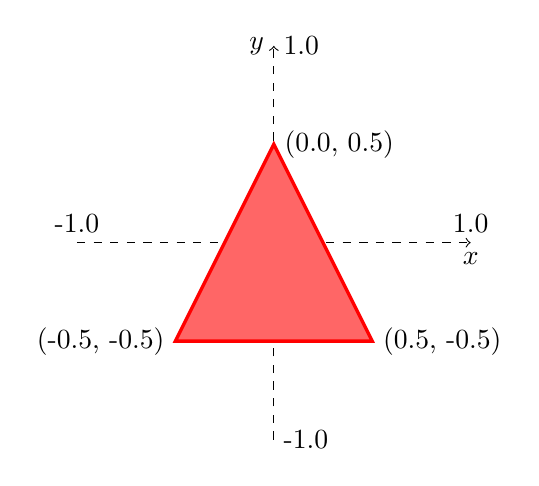
\begin{tikzpicture}[scale=2.5]
		\draw[->, dashed]
		(-1.0, 0) node[above] {-1.0} --
		(1.0, 0) node[above] {1.0} node[below] {$x$};

		\draw[->, dashed]
		(0, -1) node[right] {-1.0} --
		(0, 1) node[right] {1.0} node[left] {$y$};

		\filldraw[color=red, fill=red!60, very thick]
		(-0.5, -0.5) node[left, color=black] {(-0.5, -0.5)} --
		(0, 0.5) node[right, color=black] {(0.0, 0.5)} --
		(0.5, -0.5) node[right, color=black] {(0.5, -0.5)} --
		cycle;
	\end{tikzpicture}
\end{center}

\subsection{Array Buffer}
Per iniziare a disegnare qualcosa dobbiamo dare a WebGL delle informazioni sulla geometria
che vogliamo visualizzare.

Se volessimo disegnare un triangolo, la prima cosa che probabilmente ci verr\`a in mente
\`e specificare le coordinate $(x, y)$ dei tre vertici.

Iniziamo con il definire un array di \verb|float| contenente i nostri vertici.
\begin{lstlisting}[language=javascript]
function geometrySetup() {
	var data = new Float32Array([
		-0.5, -0.5,
		 0.0,  0.5,
		 0.5, -0.5
	]);
\end{lstlisting}
Ora vogliamo rendere questi valori visibili dalla scheda grafica. Per farlo dobbiamo metterli
in un \textbf{buffer} da cui poi verranno letti.
\begin{lstlisting}[language=javascript, firstnumber=7]
	var buffer = gl.createBuffer();
	gl.bindBuffer(gl.ARRAY_BUFFER, buffer);
	gl.bufferData(gl.ARRAY_BUFFER, data, gl.STATIC_DRAW);
\end{lstlisting}
Spieghiamo queste 3 righe di codice:
\begin{enumerate}
	\item Viene creato un buffer nella memoria della GPU.
	\item Il buffer viene associato a un target (in questo caso \verb|ARRAY_BUFFER|).
	\item I dati dell'array \verb|data| vengono caricati nel buffer.

	      L'ultimo parametro \`e un
	      suggerimento che per l'ottimizzazione. In questo caso ci dice che i dati caricati
	      nel buffer non dovrebbero variare molto. Nel caso in cui volessimo disegnare
	      qualcosa in movimento potrebbe essere una buona scelta usare \verb|DYNAMIC_DRAW|.
\end{enumerate}

\subsection{Vertex Attribute Array}
Ora per\`o dobbiamo dire al programma come leggere questi dati.
Per prima cosa dobbiamo sapere che ogni scheda video ha in memoria una sorta array in
cui si possono inserire le "\emph{istruzioni}" su come leggere i dati che abbiamo caricato
precedentemente nel buffer. Supponendo di averne $N$, allora saranno numerati da 0 a $N-1$
($N$ dipende dalla GPU).

In ciascuna cella dell'array sono presenti informazioni sui diversi attributi che pu\`o
avere ogni vertice della geometria che disegnamo. In questo caso abbiamo solo la posizione
del vertice ma in futuro potremo inserire anche altri attributi come ad esempio il colore.

Per il momenti limitiamoci a scrivere una cosa di questo tipo:
\begin{lstlisting}[language=javascript, firstnumber=10]
	gl.enableVertexAttribArray(0);
	gl.vertexAttribPointer(0, 2, gl.FLOAT, false, 8, 0);
}
\end{lstlisting}
La seconda funzione va a scrivere le informazioni necessarie a interpretare i dati nel
buffer.
\begin{itemize}
	\item Per prima cosa indichiamo in quale \textbf{posizione} dell'array degli attributi
	      vogliamo scrivere le informazioni. In questo caso 0.
	\item Il secondo parametro ci dice quanti valori devo considerare (per ciascun vertice)
	      per poter descrivere l'attributo. In questo caso abbiamo 2 dato che l'attributo
	      che vogliamo descrivere \`e la posizione del vertice (coppia $(x, y)$ di
	      coordinate).
	\item Il terzo parametro \`e semplicemente il \textbf{tipo} dei singoli valori dell'array.
	      Nel nostro caso abbiamo un array di float quindi scriviamo \verb|gl.FLOAT|.
	\item Il quarto parametro \`e la \textbf{normalizzazione} ma la vedremo pi\`u avanti.
	      Per ora lasciamolo a \verb|false|.
	\item Il quinto parametro \`e la \textbf{stride}. Indica il numero di byte che intercorre
	      tra i dati che descrivono un vertice e quello successivo. In sostanza ci dice ogni
	      quanti byte inizia la descrizione di un nuovo vertice. Nel nostro caso abbiamo 8
	      come valore perch\'e abbiamo che un vertice \`e descritto solamente dalle sue
	      coordinate spaziali $x, y$. Sono di tipo float e quindi ottengo $2 * 4 = 8$ byte
	      che dividono l'inizio di un vertice dall'altro.
	\item L'ultmo valore \`e l'\textbf{offset}. Indica quanti byte saltare prima di iniziare
	      a leggere l'array. Nel nostro caso vale 0 perch\'e iniziamo a leggere l'array
	      dall'inizio. Pi\`u avanti sar\`a utile impostare valori diversi dell'offset
	      nel caso avessimo pi\`u attributi per uno stesso vertice.
\end{itemize}
La prima funzione non fa altro che abilitare il primo slot dell'array degli attributi.
Stiamo quindi notificando il programma che al posto 0 dell'array ci sono informazioni
necessarie per interpretare i dati scritti nel buffer.

\subsection{Shader}
Ora che abbiamo comunicato alla GPU come leggere i dati nel buffer dobbiamo dargli un
metodo per disegnare la geometria che vogliamo. Per farlo utilizziamo gli \textbf{shader}.
Per scriverli si usa un linguaggio (GLSL) simile al C.

Uno shader \`e un piccolo programma che viene eseguito nella memoria della GPU ed \`e
fondamentale per la costruzione della geometria e per la fase di rendering finale.

Gli shader possono essere di due tipi: \textbf{vertex} e \textbf{fragment}.

\subsubsection{Vertex Shader}
Il vertex shader si occupa di assemblare la geometria che vogliamo disegnare.
\begin{lstlisting}[language=javascript]
function shaderSetup() {
	var vs_source =
		`attribute vec2 aPosition;
		
		void main()
		{
			gl_Position = vec4(aPosition, 0.0, 1.0);
		}`
	;
\end{lstlisting}
La variabile \verb|aPosition| ha due tipi: \verb|attribute| e \verb|vec2|. Il primo
indica che il valore deve essere preso dall'array degli attributi visto in precedenza
(dopo vediamo come fare nello specifico). Il secondo tipo indica semplicemente che
si tratta di una coppia di valori o vettore bidimensionale.

Nel \verb|main| \`e presente la variabile \verb|gl_Position|, una variabile speciale, che
indica la posizione di ci\`o che sto disegnando.

\subsubsection{Fragment Shader}
Il fragment shader si occupa della fase di rasterizzazione, in cui si va a decidere il
colore di ci\`o che viene visualizzato.
\begin{lstlisting}[language=javascript, firstnumber=8]
	var fs_source =
		`void main()
		{
			gl_FragColor = vec4(1.0, 0.0, 0.0, 1.0);
		}`
	;
\end{lstlisting}
In questo caso abbiamo solo la variabile \verb|gl_FragColor| un vettore a 4 dimensioni.
I primi 3 valori sono i valori di rosso, verde e blu, il quarto valore \`e la trasparenza.
Tutti e quattro i valori vanno da 0 a 1. Dato che abbiamo il rosso a 1, mentre il verde e
il blu sono a 0, ci aspettiamo di vedere un triangolo rosso.

\subsubsection{Compilazione}
Compiliamo i sorgenti.
\begin{lstlisting}[language=javascript, firstnumber=14]
	var vertex = gl.createShader(gl.VERTEX_SHADER);
	gl.shaderSource(vertex, vs_source);
	gl.compileShader(vertex);

	var fragment = gl.createShader(gl.FRAGMENT_SHADER);
	gl.shaderSource(fragment, fs_shader);
	gl.compileShader(fragment);
\end{lstlisting}
\newpage
Adesso dobbiamo linkare il tutto in unico programma.
\begin{lstlisting}[language=javascript, firstnumber=21]
	var program = gl.createProgram();
	gl.attachShader(program, vertex);
	gl.attachShader(program, fragment);
	gl.linkProgram(program);
	gl.useProgram(program);
\end{lstlisting}
Concludiamo con questo comando
\begin{lstlisting}[language=javascript, firstnumber=26]
	gl.bindAttribLocation(program, 0, "aPosition");
}
\end{lstlisting}
il quale indica allo shader di prendere le informazioni dalla posizione 0 dell'array degli
attributi e metterle dentro la variabile \verb|aPosition| del vertex shader. In questo caso
si tratta delle coordinate dei vertici del triangolo.

\section{Draw}
Non ci rimane che invocare le funzioni necessarie per disegnare il nostro triangolo rosso.
\begin{lstlisting}[language=javascript]
function drawTriangle() {
	gl.clearColor(1.0, 1.0, 1.0, 1.0);
	gl.clear(COLOR_BUFFER_BIT);
	gl.drawArrays(gl.TRIANGLES, 0, 3);
}
\end{lstlisting}
Le prime due funzioni colorano lo sfondo. In questo caso otterremo lo sfondo bianco.

L'ultima \`e quella che disegner\`a il triangolo. Il primo parametro dice di considerare
gruppi di 3 vertici alla volta (triangoli per l'appunto). Il secondo indica da che vertice
iniziare mentre il terzo indica il numero di vertici che voglio disegnare.

Ricoridiamoci che la funzione \verb|run| scritta all'inizio dovr\`a essere aggiornata
in questo modo:
\begin{lstlisting}[language=javascript]
function run() {
	initWebGL();
	geometrySetup();
	shaderSetup();
	drawTriangle();
}
\end{lstlisting}
Arrivati a questo punto dovremmo avere a schermo il nostro triangolo rosso su sfondo bianco.

\newpage
\section{Index Buffer}
Se volessimo disgnare un quadrato baster\`a unire due triangoli rettangoli per l'ipotenusa.

\begin{center}
	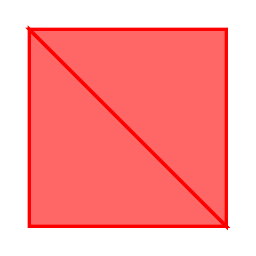
\begin{tikzpicture}[scale=2.5]
		\filldraw[color=red, fill=red!60, very thick]
		(-0.5, -0.5) --
		(-0.5, 0.5) --
		(0.5, -0.5) --
		cycle;

		\filldraw[color=red, fill=red!60, very thick]
		(-0.5, 0.5) --
		(0.5, 0.5) --
		(0.5, -0.5) --
		cycle;
	\end{tikzpicture}
\end{center}
Per farlo posso usare il metodo visto in precedenza per disegnare triangoli. Dovr\`o quindi
specificare altri tre vertici per il secondo triangolo:
\begin{lstlisting}[language=javascript]
	var data = new Float32Array([
		// primo triangolo
		-0,5, -0.5,
		-0.5,  0.5,
		 0.5,  0.5,

		// secondo triangolo
		 0.5,  0.5,
		 0.5, -0.5,
		-0.5, -0.5
	]);
\end{lstlisting}
Per disegnare il quadrato dovr\`o modificare anche la chiamata alla funzione
\verb|drawArrays|:
\begin{lstlisting}[language=javascript]
	gl.drawArrays(gl.TRIANGLES, 0, 6);
\end{lstlisting}
Adesso l'ultimo parametro \`e diventato 6 perch\'e stiamo passando sei vertici.

Cos\`i facendo otteniamo il nostro quadrato ma non \`e il modo pi\`u efficente. Notiamo
che stiamo specificando due volte i due vertici in comune tra i due triangoli. Se pensiamo
di fare un progetto pi\`u grande lo spreco in memoria \`e prestazioni potrebbe essere
significativo.

Per ottimizzare questo aspetto introduciamo un nuovo oggetto, l'\textbf{index buffer}.
L'idea \`e quella di indicizzare ogni vertice della figura geometrica che stiamo disegnando.
\begin{center}
	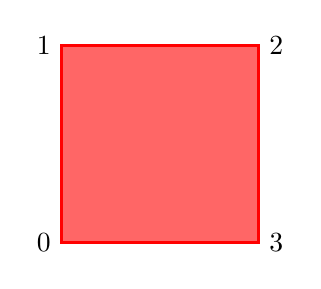
\begin{tikzpicture}[scale=2.5]
		\label{fig:index}
		\filldraw[color=red, fill=red!60, very thick]
		(-0.5, -0.5) node[left, color=black] {0} --
		(-0.5, 0.5) node[left, color=black] {1} --
		(0.5, 0.5) node[right, color=black] {2} --
		(0.5, -0.5) node[right, color=black] {3} --
		cycle;
	\end{tikzpicture}
\end{center}
Nel dettaglio, per disegnare il quadrato di prima, dovremmo specificare ogni vertice una sola
volta. L'array \verb|data| diventer\`a quindi
\begin{lstlisting}[language=javascript]
	var data = new Float32Array([
		-0.5, -0.5, // vertice 0
		-0.5,  0.5, // vertice 1
		 0.5,  0.5, // vertice 2
		 0.5, -0.5  // vertice 3
	]);
\end{lstlisting}
Ora creiamo un index buffer in questo modo
\begin{lstlisting}[language=javascript]
	var indices = new Uint16Array([
		0, 1, 2,
		2, 3, 0
	]);

	var indexBuffer = gl.createBuffer();
	gl.bindBuffer(gl.ELEMENT_ARRAY_BUFFER, indexBuffer);
	gl.bufferData(gl.ELEMENT_ARRAY_BUFFER, indices, gl.STATIC_DRAW);
\end{lstlisting}
In riferimento alla figura del quadrato con i vertici indicizzati vista in precedenza,
l'intento del codice scritto sopra \`e quello di usare i vertici $\{ 0, 1, 2 \}$ per disegnare
il primo triangolo e i vertici $\{ 2, 3, 0 \}$ per disegnare il secondo.

A questo punto non ci rimane che introdurre una nuova funzione che sostituir\`a
la \verb|drawArrays| vista in precedenza.
\begin{lstlisting}
	gl.drawElements(gl.TRIANGLES, 6, gl.UNSIGNED_SHORT, 0);
\end{lstlisting}
Vediamo meglio i parametri di questa funzione
\begin{itemize}
	\item Il primo parametro \`e un target. In questo caso abbiamo lo stesso di
	      \verb|drawArrays| ovvero \verb|TRIANGLES|.
	\item Il secondo parametro \`e il numero di indici utilizzati.
	\item Il terzo parametro \`e il tipo di dato utilizzato per rappresentare gli indici.
	      In questo caso abbiamo un \verb|Uint16Array|, quindi specifichiamo
	      \verb|UNSIGNED_SHORT|.
	\item Il quarto parametro \`e un offset che indica dopo quanti byte iniziare a leggere
	      l'array degli indici.
\end{itemize}
Ecco che in questo modo abbiamo "\emph{riciclato}" vertici comuni ai due triangoli per poter
disegnare la nostra figura (in particolare i vertici \verb|0| e \verb|2|).
